\section{Variation of Parameters}

\noindent
In this section we give a method called {\color{blue}\it variation of
parameters\/} for finding a particular solution of
\begin{equation} \label{eq:5.7.1}
P_0(x)y''+P_1(x)y'+P_2(x)y=F(x)
\end{equation}
if we know a fundamental set $\{y_1,y_2\}$ of solutions of  the
complementary equation
\begin{equation} \label{eq:5.7.2}
P_0(x)y''+P_1(x)y'+P_2(x)y=0.
\end{equation}
Having found a particular solution $y_p$ by this method, we can write
the general solution of \eqref{eq:5.7.1} as
$$
y=y_p+c_1y_1+c_2y_2.
$$

Since we need only one nontrivial solution of \eqref{eq:5.7.2} to find the
general solution of \eqref{eq:5.7.1} by reduction of order, it's natural
to ask why we're interested in variation of parameters, which requires
two linearly independent solutions of \eqref{eq:5.7.2} to achieve the same
goal. Here's the answer:

\begin{itemize}
\item If we already know two linearly independent solutions of
\eqref{eq:5.7.2} then  variation of parameters will probably  be simpler
than reduction of order.

\item Variation of parameters generalizes naturally to a method
for finding particular solutions of higher order
linear equations (Section~9.4) and  linear systems of
equations
(Section~10.7), while reduction of order doesn't.

\item Variation of parameters is a powerful theoretical tool
 used by researchers in differential equations. Although a detailed
discussion of this is beyond the scope of this book, you can get an
idea of what it means from Exercises~\ref{exer:5.7.37}--\ref{exer:5.7.39}.
 \end{itemize}

We'll now derive the method. As usual, we consider solutions of
\eqref{eq:5.7.1} and \eqref{eq:5.7.2} on an interval $(a,b)$ where  $P_0$,
$P_1$, $P_2$, and $F$ are continuous and $P_0$ has no zeros. Suppose
that $\{y_1,y_2\}$ is a fundamental set of solutions of the
complementary equation \eqref{eq:5.7.2}. We look for
 a particular solution of \eqref{eq:5.7.1} in the form
\begin{equation} \label{eq:5.7.3}
y_p=u_1y_1+u_2y_2
\end{equation}
where $u_1$ and $u_2$ are functions to be determined so that $y_p$
satisfies \eqref{eq:5.7.1}. You may not think this is a good idea, since
there are now two unknown functions to be determined, rather than one.
However, since $u_1$ and $u_2$ have to satisfy only one condition
(that $y_p$ is a solution of \eqref{eq:5.7.1}), we can impose a second
condition that produces a convenient simplification, as follows.

 Differentiating \eqref{eq:5.7.3} yields
\begin{equation} \label{eq:5.7.4}
y_p'=u_1y_1'+u_2y_2'+u_1'y_1+u_2'y_2.
\end{equation}
As our second condition on $u_1$ and $u_2$
 we require that
\begin{equation} \label{eq:5.7.5}
u_1'y_1+u_2'y_2=0.
\end{equation}
 Then  \eqref{eq:5.7.4} becomes
\begin{equation}
y_p'=u_1y_1'+u_2y_2';     \label{eq:5.7.6}
\end{equation}
that is, \eqref{eq:5.7.5} permits us to differentiate $y_p$ (once!) as if
 $u_1$ and $u_2$ are constants. Differentiating
\eqref{eq:5.7.4} yields \begin{equation} \label{eq:5.7.7}
y_p''=u_1y''_1+u_2y''_2+u_1'y_1'+u_2'y_2'. \end{equation}
(There are no terms involving $u_1''$ and $u_2''$ here, as there would
be if we hadn't required \eqref{eq:5.7.5}.) Substituting \eqref{eq:5.7.3},
\eqref{eq:5.7.6}, and \eqref{eq:5.7.7} into \eqref{eq:5.7.1} and collecting the
coefficients of $u_1$ and $u_2$ yields
$$
u_1(P_0y''_1+P_1y_1'+P_2y_1)+u_2(P_0y''_2+P_1y_2'+P_2y_2)
+P_0(u_1'y_1'+u_2'y_2')=F.
$$
As in the derivation of the method of reduction of order, the
coefficients of $u_1$ and $u_2$ here are both zero because $y_1$ and
$y_2$ satisfy the complementary equation. Hence, we can rewrite the
last equation  as
\begin{equation}\label{eq:5.7.8}
  P_0(u_1'y_1'+u_2'y_2')=F.
\end{equation}
Therefore $y_p$ in \eqref{eq:5.7.3} satisfies \eqref{eq:5.7.1} if
\begin{equation} \label{eq:5.7.9}
\begin{array}{rcl}
u_1'y_1+u_2'y_2 &=& 0  \\
u_1'y_1'+u_2'y_2' &=& \dst{F\over P_0},
\end{array}
\end{equation}
where the first equation is the same as \eqref{eq:5.7.5} and the second is
from \eqref{eq:5.7.8}.

We'll now show that you can always solve \eqref{eq:5.7.9} for $u_1'$
and $u_2'$. (The method that we use here will always work, but simpler
methods usually work when you're dealing with specific equations.) To
obtain $u_1'$, multiply the first equation in \eqref{eq:5.7.9} by $y_2'$
and the second equation by $y_2$. This yields
\begin{eqnarray*}
u_1'y_1y_2'+u_2'y_2y_2'&=& 0  \\
u_1'y_1'y_2+u_2'y_2'y_2 &=& {Fy_2\over P_0}.
\end{eqnarray*}
Subtracting the second equation from the first yields
\begin{equation} \label{eq:5.7.10}
u_1'(y_1y_2'-y_1'y_2)=-{Fy_2\over P_0}.
\end{equation}
Since $\{y_1,y_2\}$  is a fundamental set of solutions of \eqref{eq:5.7.2}
on $(a,b)$, Theorem~\ref{thmtype:5.1.6}\; implies that the Wronskian
 $y_1y_2'-y_1'y_2$  has no zeros on $(a,b)$.  Therefore we can solve
\eqref{eq:5.7.10} for $u_1'$, to obtain
\begin{equation} \label{eq:5.7.11}
u_1'=-{Fy_2\over P_0(y_1y_2'-y_1'y_2)}.
\end{equation}
We leave it to you to start from \eqref{eq:5.7.9} and show by a similar
argument that
\begin{equation} \label{eq:5.7.12}
u_2'={Fy_1\over P_0(y_1y_2'-y_1'y_2)}.
\end{equation}

We can now obtain $u_1$ and $u_2$ by integrating $u_1'$ and $u_2'$.
The constants of integration can be taken to be zero, since any choice
of $u_1$ and $u_2$ in \eqref{eq:5.7.3} will suffice.

You should not memorize \eqref{eq:5.7.11} and \eqref{eq:5.7.12}. On the
other hand, you don't want to rederive the whole procedure for every
specific problem. We recommend the a compromise:
\begin{alist}
\item % (a)
Write
\begin{equation} \label{eq:5.7.13}
y_p=u_1y_1+u_2y_2
\end{equation}
to remind yourself of what you're doing.
\item % (b)
Write the system
\begin{equation} \label{eq:5.7.14}
\begin{array}{rcl}
u_1'y_1+u_2'y_2 &=& 0  \\
u_1'y_1'+u_2'y_2' &=& \dst{F\over P_0}
\end{array}
\end{equation}
for the specific problem  you're trying to solve.
\item % (c)
Solve \eqref{eq:5.7.14} for $u_1'$ and $u_2'$ by any convenient method.
\item % (d)
Obtain $u_1$ and $u_2$ by integrating $u_1'$ and $u_2'$,
taking the constants of integration to be zero.
\item % (e)
Substitute $u_1$ and $u_2$ into \eqref{eq:5.7.13}  to obtain $y_p$.
\end{alist}

\begin{example}\label{example:5.7.1} \rm
 Find a particular
solution $y_p$ of
\begin{equation} \label{eq:5.7.15}
x^2y''-2xy'+2y=x^{9/2},
\end{equation}
given that $y_1=x$ and $y_2=x^2$ are solutions of the complementary
equation
$$
x^2y''-2xy'+2y=0.
$$
 Then find the general solution of \eqref{eq:5.7.15}.
\end{example}

\solution
We set
$$
y_p=u_1x+u_2x^2,
$$
where
\begin{eqnarray*}
u_1'x+\phantom{2}u_2'x^2&=&0\\
u_1'\phantom{x}+2u_2'x\phantom{^2}&=&{x^{9/2}\over x^2}=x^{5/2}.
\end{eqnarray*}
From the first equation, $u_1'=-u_2'x$. Substituting this into the
second equation yields $u_2'x=x^{5/2}$, so $u_2'=x^{3/2}$ and
therefore $u_1'=-u_2'x=-x^{5/2}$. Integrating and taking the constants
of integration to be zero yields
$$
u_1=-{2\over7}x^{7/2}\mbox{\quad and \quad}u_2={2\over5}x^{5/2}.
$$
Therefore
$$
y_p=u_1x+u_2x^2
=-{2\over7}x^{7/2}x+{2\over5}x^{5/2}x^2={4\over35}x^{9/2},
$$
and the general solution of  \eqref{eq:5.7.15} is
$$
y={4\over35}x^{9/2}+c_1x+c_2x^2.
$$

\begin{example}\label{example:5.7.2} \rm
 Find a particular
solution $y_p$ of
\begin{equation} \label{eq:5.7.16}
(x-1)y''-xy'+y=(x-1)^2,
\end{equation}
given that $y_1=x$ and $y_2=e^x$ are solutions of the complementary
equation
$$
(x-1)y''-xy'+y=0.
$$
 Then find the general solution of \eqref{eq:5.7.16}.
\end{example}

\solution
We set
$$
y_p=u_1x+u_2e^x,
$$
where
\begin{eqnarray*}
u_1'x+u_2'e^x&=&0\\
u_1'\phantom{x}+u_2'e^x&=&{(x-1)^2\over x-1}=x-1.
\end{eqnarray*}
Subtracting the first equation from the second yields
$-u_1'(x-1)=x-1$, so $u_1'=-1$. From this and the first equation,
$u_2'=-xe^{-x}u_1'=xe^{-x}$.
Integrating and taking the constants of integration to be zero yields
$$
u_1=-x  \mbox{\quad and \quad} u_2=-(x+1)e^{-x}.
$$
Therefore
$$
y_p=u_1x+u_2e^x
=(-x)x+(-(x+1)e^{-x})e^x=-x^2-x-1,
$$
so the general solution of \eqref{eq:5.7.16} is
\begin{equation} \label{eq:5.7.17}
y=y_p+c_1x+c_2e^x=-x^2-x-1+c_1x+c_2e^x = -x^2-1+(c_1-1)x+c_2e^x.
\end{equation}
However, since $c_1$ is an arbitrary constant, so is $c_1-1$;
therefore, we  improve the appearance of this result by
renaming the constant and writing the general solution as
\begin{equation} \label{eq:5.7.18}
y= -x^2-1+c_1x+c_2e^x.\bbox
\end{equation}

There's nothing {\color{blue}\it wrong\/} with leaving the general solution of
\eqref{eq:5.7.16} in the form \eqref{eq:5.7.17};     however, we think
you'll agree that \eqref{eq:5.7.18} is preferable. We can also view the
transition from \eqref{eq:5.7.17} to \eqref{eq:5.7.18} differently. In
this example the particular solution $y_p=-x^2-x-1$ contained the term
$-x$, which satisfies the complementary equation. We can
 drop this term and redefine $y_p=-x^2-1$, since
 $-x^2-x-1$ is a solution of \eqref{eq:5.7.16} and $x$ is a solution
of the complementary equation; hence, $-x^2-1=(-x^2-x-1)+x$
is also a solution of \eqref{eq:5.7.16}. In general, it's always
legitimate to drop linear combinations of $\{y_1,y_2\}$ from
particular solutions obtained by variation of parameters. (See
Exercise~\ref{exer:5.7.36} for a general discussion of this question.)
We'll do this in the following  examples and in the answers to
exercises that ask  for a particular solution. Therefore, don't be
concerned if your answer to such an exercise differs from ours only by
a solution of the complementary equation.

\begin{example}\label{example:5.7.3} \rm
 Find a particular solution of
\begin{equation}  \label{eq:5.7.19}
y''+3y'+2y={1\over 1+e^x}.
\end{equation}
Then find the general solution.
\end{example}

\solution

The characteristic polynomial of the complementary equation
\begin{equation} \label{eq:5.7.20}
y''+3y'+2y=0
\end{equation}
is $p(r)=r^2+3r+2=(r+1)(r+2)$, so
$y_1=e^{-x}$ and $y_2=e^{-2x}$ form a fundamental set of solutions of
\eqref{eq:5.7.20}.  We look for a particular solution of
\eqref{eq:5.7.19} in the form
$$
y_p=u_1e^{-x}+u_2e^{-2x},
$$
where
\begin{eqnarray*}
\phantom{-}u_1'e^{-x}+\phantom{2}u_2'e^{-2x}&=&0\\
-u_1'e^{-x}-2u_2'e^{-2x}&=&{1\over 1+e^x}.
\end{eqnarray*}
Adding these two equations yields
$$
-u_2'e^{-2x}={1\over1+e^x},\mbox{\quad so \quad}
u_2'=-{e^{2x}\over 1+e^x}.
 $$
From the first equation,
$$
u_1'=-u_2'e^{-x}={e^x\over 1+e^x}.
$$
Integrating by means of  the substitution $v=e^x$ and taking the
constants of integration to be zero  yields
 $$
u_1=\int{e^x\over 1+e^x}\,dx=\int {dv\over 1+v}
=\ln(1+v)=\ln(1+e^x)
$$
and
\begin{eqnarray*}
u_2&=&-\int{e^{2x}\over 1+e^x}\,dx=-\int {v\over 1+v}\,dv
=\int\left[{1\over 1+v}-1\right]\,dv \\ [2\jot]
&=&\ln(1+v)-v=\ln(1+e^x)-e^x.
\end{eqnarray*}
Therefore
\begin{eqnarray*}
y_p&=&u_1e^{-x}+u_2e^{-2x}\\
&=&[\ln(1+e^x)]e^{-x}+\left[\ln(1+e^x)-e^x\right]e^{-2x},
\end{eqnarray*}
so
$$
y_p=\left(e^{-x}+e^{-2x}\right)\ln(1+e^x)-e^{-x}.
$$
Since the last term on the right satisfies  the complementary
equation, we drop it and redefine
$$
y_p=\left(e^{-x}+e^{-2x}\right)\ln(1+e^x).
$$
The general solution of
 \eqref{eq:5.7.19} is
$$
y=y_p+c_1e^{-x}+c_2e^{-2x}=\left(e^{-x}+e^{-2x}\right)\ln(1+e^x)
+c_1e^{-x}+c_2e^{-2x}.
$$

\begin{example}\label{example:5.7.4} \rm
Solve the initial value problem
\begin{equation} \label{eq:5.7.21}
(x^2-1)y''+4xy'+2y={2\over x+1}, \quad  y(0)=-1,\quad y'(0)=-5,
\end{equation}
 given that
$$
y_1={1\over x-1}\quad\mbox{ and }\quad y_2={1\over x+1}
$$
are  solutions of the complementary
equation
$$
(x^2-1)y''+4xy'+2y=0.
$$
\end{example}

\solution
We first use variation of parameters to find a particular solution
of
$$
(x^2-1)y''+4xy'+2y={2\over x+1}
$$
on $(-1,1)$ in the form
$$
y_p={u_1\over x-1}+{u_2\over x+1},
$$
where
\begin{eqnarray}
\phantom{-}{u_1'\over\phantom{(}x-1\phantom{)^2}}+{u_2'\over
\phantom{(}x+1\phantom{)^2}}&=&0\label{eq:5.7.22}\\
-{u_1'\over(x-1)^2}-{u_2'\over(x+1)^2}&=&{2\over(x+1)(x^2-1)}.\nonumber
\end{eqnarray}
Multiplying the first equation by $1/(x-1)$ and adding the result to
the second equation yields
\begin{equation} \label{eq:5.7.23}
\left[{1\over x^2-1}-{1\over(x+1)^2}\right]u_2'={2\over(x+1)(x^2-1)}.
\end{equation}
Since
$$
\left[{1\over x^2-1}-{1\over(x+1)^2}\right]={(x+1)-(x-1)\over(x+1)(x^2-1)}
={2\over(x+1)(x^2-1)},
$$
\eqref{eq:5.7.23} implies that $u_2'=1$. From \eqref{eq:5.7.22},
$$
u_1'=-{x-1\over x+1}u_2'=-{x-1\over x+1}.
$$
Integrating and taking the constants of integration to be zero yields
\begin{eqnarray*}
u_1&=&-\int{x-1\over x+1}\,dx=-\int{x+1-2\over x+1}\,dx \\
&=&\int\left[{2\over x+1}-1\right]\,dx=2\ln(x+1)-x
\end{eqnarray*}
and
$$
u_2=\int\,dx=x.
$$
Therefore
\begin{eqnarray*}
y_p&=&{u_1\over x-1}+{u_2\over x+1}=\left[2\ln(x+1)-x\right]{1\over
x-1}
+x{1\over x+1} \\
&=&{2\ln(x+1)\over x-1}+x\left[{1\over x+1}-{1\over x-1}\right]
={2\ln(x+1)\over x-1}-{2x\over(x+1)(x-1)}.
\end{eqnarray*}
However, since
$$
{2x\over(x+1)(x-1)}=\left[{1\over x+1}+{1\over x-1}\right]
$$
is a solution of the complementary equation, we redefine
$$
y_p={2\ln(x+1)\over x-1}.
$$
Therefore  the general solution of  \eqref{eq:5.7.24} is
\begin{equation} \label{eq:5.7.24}
y={2\ln(x+1)\over x-1}+{c_1\over x-1}+{c_2\over x+1}.
\end{equation}
Differentiating this yields
$$
y'={2\over
x^2-1}-{2\ln(x+1)\over(x-1)^2}-{c_1\over(x-1)^2}-{c_2\over(x+1)^2}.
$$
Setting $x=0$ in the last two equations and imposing the initial conditions
$y(0)=-1$ and $y'(0)=-5$ yields the system
\begin{eqnarray*}
-c_1+c_2&=&-1\phantom{.}\\
-2-c_1-c_2&=&-5.
\end{eqnarray*}
The solution of this system is $c_1=2,\,c_2=1$.  Substituting
these into
\eqref{eq:5.7.24} yields
\begin{eqnarray*}
y&=&{2\ln(x+1)\over x-1}+{2\over x-1}+{1\over x+1}\\
&=&{2\ln(x+1)\over x-1}+{3x+1\over x^2-1}
\end{eqnarray*}
as the solution of  \eqref{eq:5.7.21}. Figure~\ref{figure:5.7.1} is a graph
of the solution.

\begin{figure}[tbp]
  \centering
  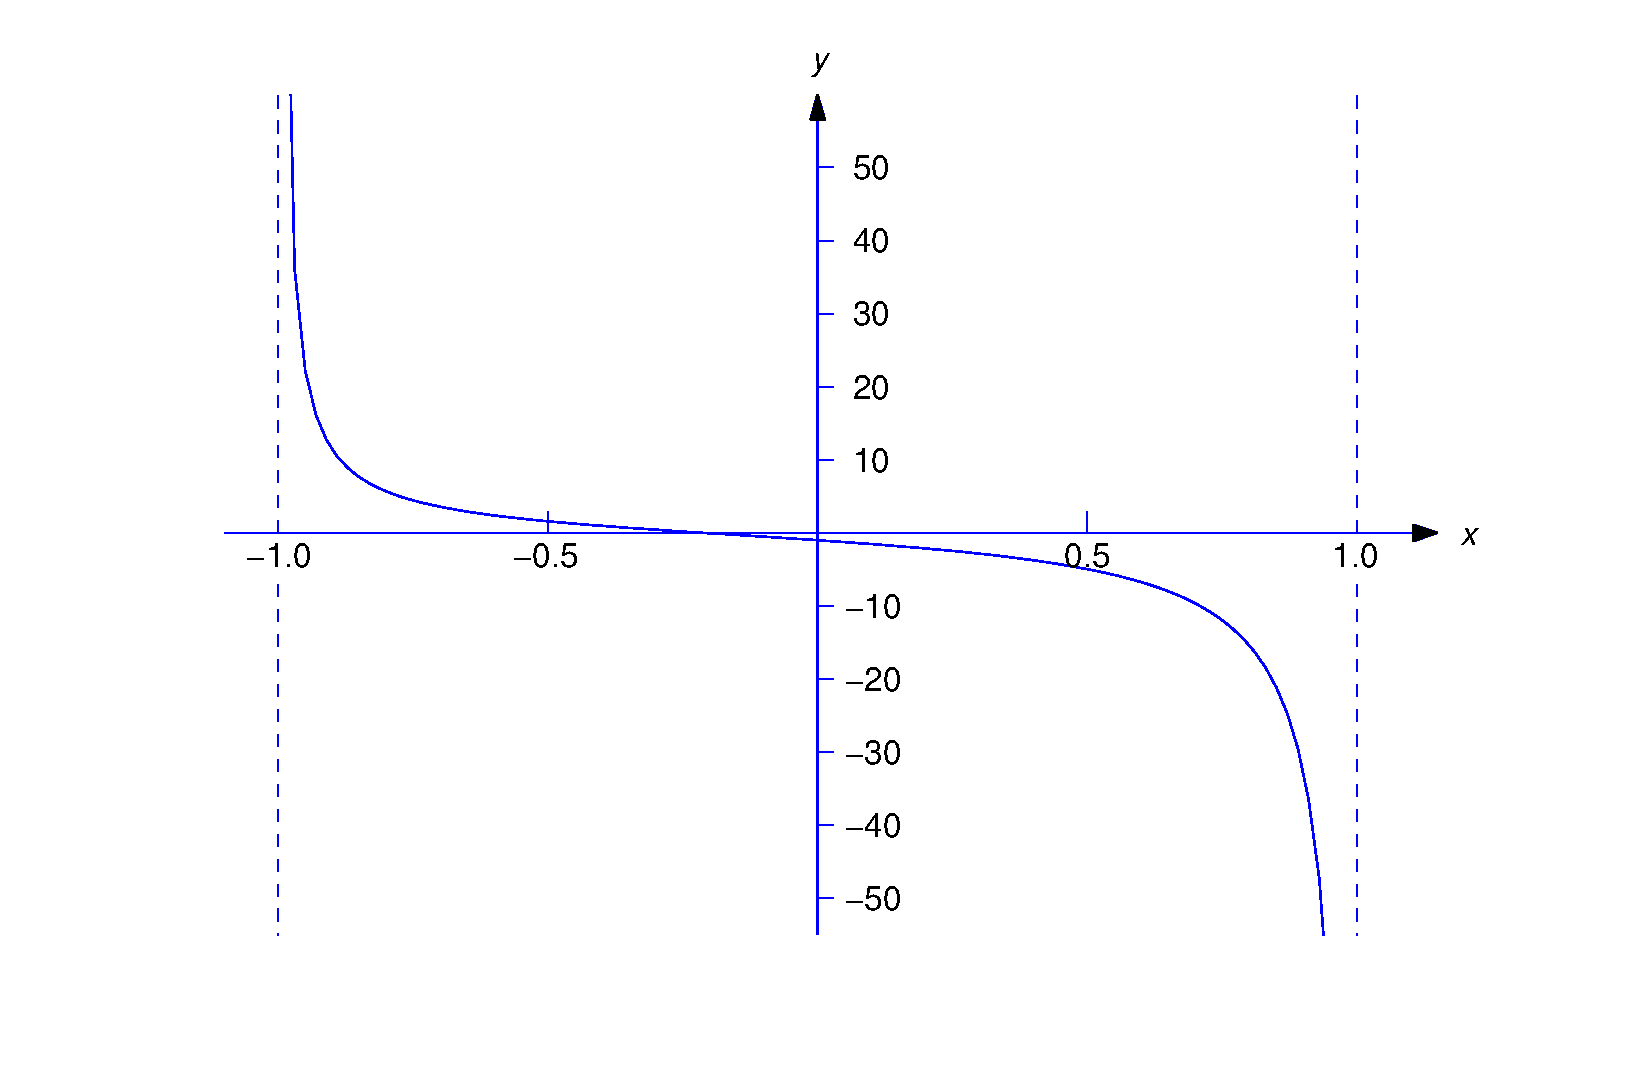
\includegraphics[bb=-78 148 689 643,width=5.67in,height=3.66in,keepaspectratio]{fig050701}
\color{blue}
  \caption{ $y=\dst{2\ln(x+1)\over x-1}+{3x+1\over x^2-1}$}
  \label{figure:5.7.1}
\end{figure}

\boxit{Comparison of Methods}

\noindent
We've now considered three methods
for solving  nonhomogeneous linear equations: undetermined
coefficients, reduction of order, and variation of parameters. It's
natural to ask which method is best for a given problem. The method of
undetermined coefficients should be used for constant coefficient
equations with forcing functions that are linear combinations of
polynomials multiplied by functions of the form $e^{\alpha x}$,
$e^{\lambda x}\cos \omega x$, or $e^{\lambda x}\sin \omega x$.
Although the other two methods can be used to solve such problems,
they will be more difficult except in the most trivial cases, because
of the integrations involved.

If the equation isn't  a constant coefficient equation or the forcing
function isn't  of the form just specified,  the method of
undetermined coefficients does not apply and the choice is necessarily
between the other two methods. The case could be made that reduction
of order is better because it requires only one solution of the
complementary equation while variation of parameters requires two.
However, variation of parameters will probably be easier if you
already know a fundamental set of solutions of the complementary
equation.

\exercises
 In Exercises~\ref{exer:5.7.1}--\ref{exer:5.7.6} use variation of
parameters to find a particular solution.

\begin{exerciselist}

\begin{tabular}[t]{@{}p{168pt}@{}p{168pt}}
\item\label{exer:5.7.1} $y''+9y=\tan 3x$
&\vspace*{10pt}  \item\label{exer:5.7.2} $y''+4y=\sin 2x\sec^2 2x$
\end{tabular}

\begin{tabular}[t]{@{}p{168pt}@{}p{168pt}}
\item\label{exer:5.7.3}  $y''-3y'+2y=\dst{4\over 1+e^{-x}}$
&  \item\label{exer:5.7.4} $y''-2y'+2y=3e^x \sec x$
\end{tabular}

\begin{tabular}[t]{@{}p{168pt}@{}p{168pt}}
\item\label{exer:5.7.5} $y''-2y'+y=14x^{3/2}e^x$
&\vspace*{-5pt} \item\label{exer:5.7.6} $y''-y=\dst{4e^{-x}\over
1-e^{-2x}}$
\end{tabular}
\newpage

\exercisetext{In Exercises \ref{exer:5.7.7}--\ref{exer:5.7.29} use variation
of parameters to find a particular solution, given the solutions
$y_1$, $y_2$ of the complementary equation.}

\item\label{exer:5.7.7}
$x^2y''+xy'- y=2x^2+2;   \quad y_1=x,
\quad y_2=\dst{1\over x}$

\item\label{exer:5.7.8}
$\dst{xy''+(2-2x)y'+(x-2)y=e^{2x};   \quad y_1=e^x,
\quad y_2={e^x\over x}}$

\item\label{exer:5.7.9}
$4x^2y''+(4x-8x^2)y'+(4x^2-4x-1)y=4x^{1/2}e^x, \quad   x > 0$;
\newline $y_1=x^{1/2} e^x,\;  y_2=x^{-1/2}e^x$

\item\label{exer:5.7.10}
$y''+4xy'+(4x^2+2)y=4e^{-x(x+2)};\quad   y_1=e^{-x^2},
\quad y_2=xe^{-x^2}$

\item\label{exer:5.7.11}
$x^2y''-4xy'+6y=x^{5/2},\, x > 0;\quad  y_1=x^2,\;  y_2=x^3$

\item\label{exer:5.7.12}
$x^2y''-3xy'+3y=2x^4\sin x; \quad  y_1=x,\;  y_2=x^3$

\item\label{exer:5.7.13}
$(2x+1)y''-2y'-(2x+3)y=(2x+1)^2e^{-x}; \quad  y_1=e^{-x},
\quad y_2=xe^x$

\item\label{exer:5.7.14}
$4xy''+2y'+y=\sin\sqrt x; \quad  y_1=\cos\sqrt x,
\quad y_2=\sin\sqrt x$

\item\label{exer:5.7.15}
$xy''-(2x+2)y'+(x+2)y=6x^3e^x;\quad  y_1=e^x,\quad  y_2=x^3e^x$

\item\label{exer:5.7.16}
$x^2y''-(2a-1)xy'+a^2y=x^{a+1}; \quad  y_1=x^a,
\quad y_2=x^a \ln x$

\item\label{exer:5.7.17}
$x^2y''-2xy'+(x^2+2)y=x^3\cos x; \quad  y_1=x\cos x,
\quad y_2=x\sin x$

\item\label{exer:5.7.18}
$xy''-y'-4x^3y=8x^5;\quad  y_1=e^{x^2},\;  y_2=e^{-x^2}$

\item\label{exer:5.7.19}
$(\sin x)y''+(2\sin x-\cos x)y'+(\sin x-\cos x)y=e^{-x}; \quad
y_1=e^{-x},\quad y_2=e^{-x}\cos x$

\item\label{exer:5.7.20}
$4x^2y''-4xy'+(3-16x^2)y=8x^{5/2}; \quad  y_1=\sqrt xe^{2x},\;  y_2=\sqrt
xe^{-2x}$

\item\label{exer:5.7.21}
$ 4x^2y''-4xy'+(4x^2+3)y=x^{7/2}; \quad  y_1=\sqrt x\sin x,\;
y_2=\sqrt x\cos x$

\item\label{exer:5.7.22}
$x^2y''-2xy'-(x^2-2)y=3x^4;\quad  y_1=xe^x,\;  y_2=xe^{-x}$

\item\label{exer:5.7.23}
$x^2y''-2x(x+1)y' +(x^2+2x+2)y=x^3e^x;   \quad y_1=xe^x, \quad y_2=x^2e^x$

\item\label{exer:5.7.24}
$x^2y''-xy'-3y=x^{3/2};  \quad y_1=1/x, \quad y_2=x^3$

\item\label{exer:5.7.25}
$x^2y''-x(x+4)y'+2(x+3)y=x^4e^x;  \quad y_1=x^2, \quad y_2=x^2e^x$

\item\label{exer:5.7.26}
$x^2y''-2x(x+2)y'+(x^2+4x+6)y=2xe^x;  \quad y_1=x^2e^x, \quad y_2=x^3e^x$

\item\label{exer:5.7.27}
$x^2y''-4xy'+(x^2+6)y=x^4;  \quad y_1=x^2\cos x, \quad y_2=x^2\sin x$

\item\label{exer:5.7.28}
 $(x-1)y''-xy'+y=2(x-1)^2e^x;  \quad y_1=x, \quad y_2=e^x$

\item\label{exer:5.7.29}
$4x^2y''-4x(x+1)y'+(2x+3)y=x^{5/2}e^x;   \quad
y_1=\sqrt x, \quad y_2=\sqrt xe^x$

\exercisetext{In Exercises \ref{exer:5.7.30}--\ref{exer:5.7.32} use variation
of parameters to solve the initial value problem, given
$y_1$, $y_2$ are solutions of the complementary equation.}

\item\label{exer:5.7.30}
$(3x-1)y''-(3x+2)y'-(6x-8)y=(3x-1)^2e^{2x}, \quad   y(0)=1,\;
y'(0)=2$;

$y_1=e^{2x},\;  y_2=xe^{-x}$

\item\label{exer:5.7.31}
$(x-1)^2y''-2(x-1)y'+2y=(x-1)^2, \quad   y(0)=3,\quad   y'(0)=-6$;

$y_1=x-1$,\;
$y_2=x^2-1$

\item\label{exer:5.7.32}
$(x-1)^2y''-(x^2-1)y'+(x+1)y=(x-1)^3e^x, \quad  y(0)=4,\quad y'(0)=-6$;

$y_1=(x-1)e^x,\quad y_2=x-1$

\newpage

\exercisetext{In Exercises \ref{exer:5.7.33}--\ref{exer:5.7.35} use variation
of parameters to solve the initial value problem and graph the
solution, given that $y_1$, $y_2$ are solutions of the complementary
equation.}

\item\label{exer:5.7.33} \CGex
$\dst{(x^2-1)y''+4xy'+2y=2x, \quad   y(0)=0,\;  y'(0)
=-2; \quad   y_1={1\over x-1},\;  y_2={1\over x+1}}$

\item\label{exer:5.7.34} \CGex
$\dst{x^2y''+2xy'-2y=-2x^2, \quad   y(1)=1,\;  y'(1)=
-1; \quad  y_1=x,\;  y_2={1\over x^2}}$

\item\label{exer:5.7.35} \CGex
$(x+1)(2x+3)y''+2(x+2)y'-2y=(2x+3)^2, \quad  y(0)=0,\quad y'(0)=0$;
\newline $y_1=x+2,\quad y_2=\dst{1\over x+1}$

\item\label{exer:5.7.36}
Suppose
$$
y_p=\overline y+a_1y_1+a_2y_2
$$
is a particular solution of
$$
P_0(x)y''+P_1(x)y'+P_2(x)y=F(x),
\eqno{\rm (A)}
$$
where  $y_1$  and $y_2$ are  solutions of the complementary equation
$$
P_0(x)y''+P_1(x)y'+P_2(x)y=0.
$$
Show that $\overline y$  is also a solution of  (A).

\item\label{exer:5.7.37}
Suppose $p$,  $q$, and $f$ are continuous
on $(a,b)$ and let $x_0$ be in $(a,b)$. Let
$y_1$ and $y_2$ be the  solutions of
$$
y''+p(x)y'+q(x)y=0
$$
such that
$$
y_1(x_0)=1, \quad y_1'(x_0)=0, \quad y_2(x_0)=0, \quad
y_2'(x_0)=1.
$$
Use variation of parameters to show that the solution of the initial
value problem
$$
y''+p(x)y'+q(x)y=f(x), \quad   y(x_0)=k_0,\;  y'(x_0)=k_1,
$$
is
$$
\begin{array}{rcl}
y(x) &=& k_0y_1(x)+k_1y_2(x) \\
& & \dst \qquad+\int^x_{x_0}\left(y_1(t)y_2(x)-
y_1(x)y_2(t)\right)
f(t)\exp\left(\int^t_{x_0}p(s)\,ds\right)\,dt.
\end{array}
$$
\hint{Use Abel's formula for the Wronskian of $\{y_1,y_2\}$, and
integrate $u_1'$ and $u_2'$ from $x_0$ to $x$.} Show also that
$$
\begin{array}{rcl}
y'(x) &=& k_0y_1'(x)+k_1y_2'(x) \\[2\jot]
& & \dst \qquad+\int^x_{x_0}\left(y_1(t)y_2'(x)-y_1'(x)y_2(t)
\right)f(t)\exp\left(\int^t_{x_0}p(s)\,ds\right)\,dt.
\end{array}
$$

\item\label{exer:5.7.38}
Suppose $f$ is continuous on an open interval
that contains $x_0=0$.
Use variation of parameters to
find a formula for the solution of the initial value problem
$$
y''-y=f(x), \quad  y(0)=k_0,\quad y'(0)=k_1.
$$

\item\label{exer:5.7.39}
Suppose $f$ is continuous on
$(a,\infty)$, where $a<0$, so $x_0=0$ is in $(a,\infty)$.

\begin{alist}
\item % (a)
Use variation of parameters to
find a formula for the solution of the initial value problem
$$
y''+y=f(x), \quad  y(0)=k_0,\quad y'(0)=k_1.
$$
\hint{You will need the addition formulas for the sine and cosine:
\begin{eqnarray*}
\sin(A+B)&=&\sin A\cos B+\cos A\sin B\\
\cos(A+B)&=&\cos A\cos B-\sin A\sin B.
\end{eqnarray*}}
\end{alist}

For the rest of this exercise assume that the improper
integral
$\int_{0}^\infty f(t)\,dt$ is absolutely convergent.

\begin{alist}[start=2]
\item % (b)
Show that if $y$ is a solution of
$$
y''+y=f(x)
\eqno{\rm (A)}
$$
 on $(a,\infty)$, then
 $$
\lim_{x \to \infty}\left(y(x)-A_0\cos x-A_1\sin x\right)=0
\eqno{\rm (B)}
$$
and
$$
\lim_{x\to\infty}\left(y'(x)+A_0\sin x-A_1\cos x\right)=0,
\eqno{\rm (C)}
$$
where
$$
A_0=k_0-\int_0^\infty f(t)\sin t\,dt\mbox{\quad and \quad}
A_1=k_1+\int_0^\infty f(t)\cos t\,dt.
$$
\hint{Recall from calculus that if $\int_0^\infty f(t)\,dt$
converges absolutely, then $\lim_{x\to\infty}\int_x^\infty
|f(t)|\,dt~=~0$.}

\item % (c)
Show that if $A_0$ and $A_1$ are arbitrary constants, then there's a
unique solution of $y''+y=f(x)$ on $(a,\infty)$ that satisfies
(B)  and (C).
\end{alist}

\end{exerciselist}

